\documentclass[a4paper,12pt]{article}
\usepackage[top=2cm,left=4cm,right=4cm,bottom=2cm]{geometry}
\RequirePackage[brazil]{babel}
\usepackage[brazil]{babel}
\usepackage[utf8]{inputenc}
\usepackage{cite}
\usepackage{verbatim}
\usepackage{latexsym}
\usepackage{amsfonts}
\usepackage{amssymb}
\usepackage{graphicx}
\usepackage{hyperref}

% – inicio codigo fonte
\usepackage{listings}

\lstset{numbers=left,
stepnumber=1,
firstnumber=1,
numberstyle=\tiny,
extendedchars=true,
breaklines=true,
frame=tb,
basicstyle=\footnotesize,
stringstyle=\ttfamily,
showstringspaces=false
}
\renewcommand{\lstlistingname}{Code}
\renewcommand{\lstlistlistingname}{java}
% – fim codigo fonte

% Title Page
\title{Transformação Data Warehouse para MapReduce no projeto ProInfoData}

\author{Tiago Rodrigo Kepe e Felipe Bolsi}


\begin{document}
\maketitle

\section{\textbf{Introdução}}

O projeto ProInfoData tem como objetivo monitorar diariamente os computadores de
todas as escolas públicas do Brasil. O monitoramento visa disponibilizar dados
para que o MEC e a sociedade acompanhem o estado de funcionamento dos
computadores. Inicialmente este parque computacional foi estimado em 500.000
computadores, atualmente, essa estimativa aumentou para mais de 1.000.000 de
máquinas, a tendência é que continue crescendo como tempo.
 
Para atender esta demanda de máquinas o sistema foi estruturado da
seguinte forma: todo computador de escola pública brasileira terá um agente (cliente)
que diariamente envia informações de uso e de hardware para o servidor central,
além das informações do uso de rede que foram incluídas recentemente. O servidor
tem duas camadas: o WebService que recebe informações dos agentes e as armazena
no Banco de Dados (BD). Essa arquitetura pode ser visualizada na fugura \ref{arquiteturaBD}
seguir:\newline

\begin{figure}[ht]
  \centering
  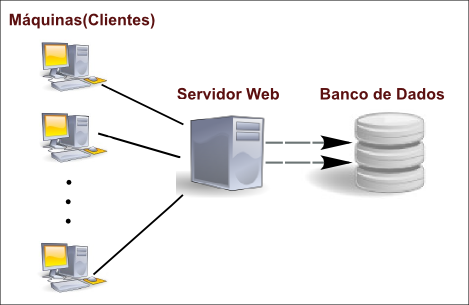
\includegraphics[width=200px,height=150px]{img/arq-bd.png}
  \caption{Visão geral da Arquitetura do ProInfoData}
  \label{arquiteturaBD}
\end{figure}

Como Sistema de Gerenciamento de Banco de Dados (SGBD) foi escolhido um SGBD
relacional, um dos motivos dessa escolha é porque o modelo relacional facilita
na associação dos dados. Para comportar o volume de dados gerado foi necessário
desenvolver uma arquitetura de armazenamento robusta e escalável. A arquitetura
proposta foi baseada em armazém de dados (Data Warehouse - DW) que é direcionada
às operações de leitura, favorecendo a análise de grandes volumes de dados e a
geração de relatórios complexos, entraremos em mais detalhes no capítulo 2.

No entanto, com o aumento emergente do número de máquinas e com o acréscimo das
informações do uso de rede, o volume de dados tornou-se extremamente grande, fato que 
nos levou a propor um nova solução para o armazenamento dos dados e para realização
das consultas disponíveis no \footnote {\href {http://seed.c3sl.ufpr.br/seed/attendance/index.html}
{portal do projeto}}.

A solução que proposmos baseia-se em uma tecnologia emergente, chamada MapReduce.
Essa solução mostrou-se eficiente em diversas implementações, a mais conhecida é
o sistema de armazenamento e busca do Google, ver \cite{MapReduceGoogle} ou
\footnote{\href {http://labs.google.com/papers/mapreduce.html} {http://labs.google.com/papers/mapreduce.html}}.

Acreditamos que o grande desafio dessa solução será a transformação do modelo
relacional para um modelo MapReduce.

No capítulo 2 descrevemos com mais detalhes o conceito de Data Warehouse e a arquitetura
do projeto ProInfoData. No capítulo 3 descrevemos o conceito de MapReduce, as 
tecnologias que serão utilizadas Hive e Hadoop e porque utlizar MapReduce no 
ProInfoData. No capítulo 4 deparamos com nosso grande desafio em propor um método de 
transformação de Data Warehouse para MapReduce. Enfim, no capítulo 5 chegamos as
conclusões dessa monografia.

\section{\textbf{Data Warehouse}}

Segundo Silberschatz e Korth \cite{Silber}“As consultas ao banco de dados normalmente 
são projetadas para extrair informações específicas, como saldo de um conta ou a soma
dos saldos de conta de um cliente. Porém, consultas projetadas para ajudar a 
formular um estratégia corporativa normalmente exigem a agregação em um escala
muito maior e incluem análise estatística não expressa facilmente com os 
recursos da SQL que já vimos anteriormente. Essas cosultas normalmente precisam 
acessar dados vindos de várias origens.”

Um DW é um repositório de dados oriundos de várias origens e armazenados sob um
banco de dados comum e que, normalmente, será mantido por um longo período de
tempo, permitindo acesso a dados históricos. Diferente dos bancos de dados
transacionais, o DW têm a característica distinta direcionada principalmente ao
suporte para tomada de decisões, segundo Navathe\cite{Navathe}. Os dados armazenados no
DW são submetidos a análises e agregações complexas, por isso, ele é um banco de
dados direcionado a consultas e análise de dados. Também é possível utilizar
técnicas para descobrir regras e padrões a partir dos dados, facilitando, assim,
a tomada de decisão. As informações são de alto nível obtidas a partir de dados
detalhados armazenados nele.

A modelagem de dados dos DW é baseada em modelos multidimensionais que 
aproveitam informações dos dados para visualização em estruturas denominadas
cubos, os cubos também são conhecidos como matrizes multidimensionais, na
representação em matrizes o desempenho pode ser muito melhor do que em modelos
relacionais, além de facilitar no processamento analítico on-line (OLAP – online
analytical processing) e na visualização dos dados.

Nesse modelo multidimensional são definidas tabelas de dimensão e tabelas fatos,
as tabelas de dimensão armazenam dados não voláteis, isto é, dados que não são
alterados frequentemente com o tempo, já as tabelas fatos armazenam dados
voláteis que são alterados constantemente e estão relacionadas as tabelas de
dimensão.

No DW os dados são extraídos de vários bancos de dados e podem estar em 
esquemas diferentes. É parte da tarefa dele agrupar toda a informação em um
único esquema.

Existem diferentes formas de manter um DW atualizado. No modelo mais
comum, a coleta de dados é orientada pela fonte, as fontes transmitem os novos 
dados. Segundo Ramakrishnan \cite{Rama} essa transmissão de dados é estipulada para
ocorrer de forma contínua para manter o repositório mais atualizado possível em
relação as suas diversas fontes. Uma outra forma possível é que a coleta dos
dados seja orientada pelo DW. Nesse modelo é enviada uma requisição as fontes
sempre que seja necessário atualizar a base central. Ramakrishnan \cite{Rama}
menciona que outra forma é a de reconstrução total da base do DW periodicamente.
Apesar de ser uma abordagem mais simples, ela não é eficiente, pois deve tratar
de grandes quantidades de dados todas as vezes em que a reconstrução for realizada.

Vale observar que em nenhuma das abordagens a base central de dados estará 
sempre atualizada em relação as todas as suas fontes. Uma forma de contornar esse
problema é a atualização em duas fases, onde as modificações feitas nas bases 
são então replicadas no DW. Mas essa abordagem torna todo o processo
muito caro em termos computacionais, segundo Ramakrishnan \cite{Rama}.

Em geral essa pequena desatualização não significa um problema para os sistemas
de suporte a decisão.

\subsection{\textbf{Data Mart}}

Data Mart (DM) é um subconjunto de dados do DW. O conjunto de DM agrupa dados
específicos de um determinado assunto ou sumariza os dados para uma determinada
finalidade, ou seja, consiste em criar dentro do DW um conjunto de dados
agregados ou sumarizados com diversos objetivos, mas principalmente em
facilitar a mineração de dados, focando na agregação para melhorar o desempenho
das consultas mais comuns ou frequentes.

Segundo Navathe \cite{Navathe}, para fazer a análise de dados mais eficiente,
o DW deve ter uma coleção de dados agregados ou sumarizados. 

No ProInfoData foram definidos gráficos e relatórios para o MEC e a sociedade
consultarem no portal do projeto, com base nessas consultas foram criados DMs
específicos para atender essa demanda, como veremos a seguir.

\subsection{\textbf{Arquiterura do Banco de Dados no ProInfoData}}

No BD do ProInfoData existem três etapas essenciais que podemos chamar de
grandes transações: carregamento, armazenamento e leitura de dados. O
carregamento consiste em receber e consolidar os dados no DW, o armazenamento é
o próprio histórico de dados do DW e a etapa de leitura organiza os dados para
otimizar as consultas. Essas etapas são implementadas em três componentes:
staging area, DW e Data Marts.

A staging area é uma tabela de armazenamento temporário, ela é responsável por
receber os dados dos clientes sem nenhuma manipulação, esses dados são inseridos
pelo servidor webservice, eles são armazenados temporariamente e após o
carregamento da staging area, são extraídos, transformados e consolidados no DW,
então são retirados da staging area. Com os dados armazenados no DW, eles,
finalmente, são sumarizados e agregados no conjundo de DM que foi projetado para
otimizar as consultas.

O DW do ProInfoData é composto por tabelas de dimensão que armazenam dados com
pouca atualização, foram criadas para armazenar informações das escolas, máquinas
e catálogo de hardware. Também é composto por tabelas fatos que são atualizadas
diariamente, essas tabelas armazenam informações de disponibilidade, inventário
de hardware e consumo de banda de rede.

O conjunto de DM é formado por quatro Data Marts: um DM para classificar a
disponibilidade das máquinas por cores. Outro DM agrupa por escola a
disponibilidade das máquinas. Existe outro para agregar informações de hardware
e um para detectar alteração de hardware.

%\textbf{Talvez inserir uma imagem da arquitetura do BD????}\\

Cada componente descrito têm sua complexidade de arquitetura, carregamento e
armazenamento. Por isso, em todos esses componentes foram realizados testes de
desempenho, utilizando uma metodologia baseada em um modelo incremental de
hardware e software. O objetivo é avaliar o sistema partindo de um ambiente
menos complexo para o mais complexo, usando cargas intermediárias até o ponto
limite do sistema. Com isso, além de encontrar a carga máxima que o sistema
suporta, fornece também resultados parciais que facilitam a avaliação de
estresse de hardware. Os testes de escrita no BD mostraram que a arquitetura
proposta chega a atender 334 transações por segundo. Já os testes de consulta
alcançou o número de 142 transações por segundo. Com estes resultados, a
arquitetura mostrou-se eficiente, atendendo as conexões e as consultas de dados
esperadas.

Entretanto, um ponto crucial do BD não entrou nessa bateria de testes que é o
carregamento dos dados para o DW e depois a agregação dos dados no conjunto de
DM. O carregamento é considerado crucial porque foi determinado um período máximo
para executá-lo que é de oito horas (entre 00h:00m até 8h:00m) porque nesse horário
o número de consultas é relativamente menor e consequentemente o impacto no BD é
menor. Além disso, os dados tem um delay de um dia, ou seja, os dados no DW são
sempre atualizados do dia anterior e não do dia atual. 

O carregamento é realizado por funções de carregamento executadas no SGBD,
realizam as junções, sumarizações e agregações necessárias. Essa etapa não
entrou nos testes porque depende dos dados já inseridos no BD, como a cada dia
são inseridos mais dados, o carregamento tende a demorar mais e, assim, aumenta
gradualmente o tempo de execução conforme cresce o volume de dados.

O desempenho das funções de carregamento depende da quantidade de dados armazenados
no BD, o volume de dados cresce diariamente, por isso, não é difícil de perceber
que o carregamento chegará ao ponto de demorar mais de oito horas para finalizar,
ocasionando maior demora na realização de consultas no BD.

Por isso, torna-se necessário usar novas tecnologias para resolver esse tipo
problema.


\section{\textbf{MapReduce}}

MapReduce é um framework criado para analisar uma grande quantidade de dados. Os
dados são divididos e designados a um conjunto de máquinas, denominado
cluster de computadores. Tem por objetivo melhorar o desempenho na performance
obtida pelo paralelismo, omitindo toda a complexidade de modo que o usuário
foque no problema principal, que é o processamento dos dados.

O modelo MapReduce é composto por duas fases, a de mapeamento dos dados e
redução. Para execução dessas fases o framework designa uma das
máquinas do cluster como master; essa máquina então define um conjunto de
máquinas para desempenhar a função de mapeamento e um outro conjunto para
executar a tarefa de redução. Na primeira fase a máquina master tem a função de
dividir os dados de entrada em várias partes menores e então designar cada parte
a uma máquina que estará desempenhando a atividade de mapeamento. Após o término
dessa fase inicia-se a fase de redução. Nessa segunda fase a máquina master
notificará as máquinas que desempenham a atividade de redução sobre a
localização dos dados produzidos pela fase anterior, para que os dados sejam
condensados em informações úteis para que possam ser interpretados e utilizados
para o fim necessário. Podemos ver a execução na figura \ref{MapReduce}.

\begin{figure}[ht]
  \centering
  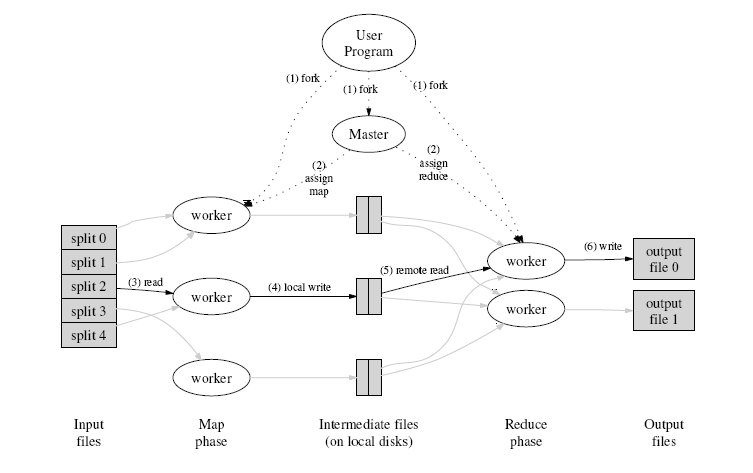
\includegraphics[width=400px,height=400px]{img/mapreduce.png}
  \caption{Visão geral da execução do framework MapReduce\newline
  Fonte: MapReduce: Simplified Data Processing on Large Clusters (2004, p. 3)}
  \label{MapReduce}
\end{figure}

Cada uma dessas fases, a de mapeamento e redução, implementa uma função, Map e 
Reduce respectivamente, ambas funções são implementadas pelo usuário.

A função Map recebe como entrada um par chave-valor. Com o par serão realizadas
as operações definidas (operações de Map e Reduce), e será produzido como saída
uma lista de pares chave-valor intermediárias. Com a conclusão dessa fase o
framework agrupará todos os valores associados a mesma chave, partindo para a
próxima fase, que utiliza a função Reduce.

A função Reduce recebe como entrada o par chave-lista de valores associada a
chave. O objetivo dessa função é realizar tarefas para agrupar ainda mais os
valores associados a mesma chave, gerando, normalmente, uma única saída.

Algumas variações do modelo são possíveis para que ele se adapte melhor as
características dos dados analisados e operações realizadas pelas funções Map e
Reduce, visando uma melhor performance na utilização do modelo. 

\subsection{\textbf{Hadoop}}

Hadoop \cite{hadoop} é um framework que permite o processamento de dados em
larga escala em clusters de computadores. Oferece um mecanismo de distribuição
dos dados em um Sistema de Arquivo Distribuído (Hadoop Distributed File System - HDFS)
ver \cite{hdfs}. Também oferece uma interface para implementar as funções de Map e 
Reduce o que facilita a programação.

As premissas do MapReduce consiste na simplificação do armazenamento, comparada
as estruturas de armazenamento do SGBD, o armazenamento utilizado deve ser
simples e normalmente armazenar uma chave e um valor para os dados.

O Hadoop pode ser instalado em três modos: Standalone, Pseudo-Distributed e
Fully-Distributed. A primeira é útil para testar a aplicação e depurar o código,
e roda como um único processo Java. O modo Pseudo-Distributed, assim como no
Standalone, é executado em apenas uma máquina, porém cada daemon do Hadoop roda
em um processo distinto. Já o modo Fully-Distributed é utilizado em sistemas de
produção, realmente distribuídos.	

Preocupações com falhas de hosts no meio de processamento de tarefas são
desconsideradas. Todos os problemas de distribuição ficam a cargo do framework.

\subsection{\textbf{Hive}}
Hive \cite{hive} é uma infra-estrutura de data warehouse construída em cima do
Hadoop. 

Ele suporta convenientemente a análise de grandes conjuntos de dados armazenados
em sistemas de arquivos compatíveis com o Hadoop,  como exemplo o sistema de
arquivos  da Amazon S3 \cite{amazon}. Ele fornece uma linguagem SQL-like chamado HiveQL
mantendo total apoio para o MapReduce. Para acelerar consultas, fornece índices
como o índice de bitmap. Um exemplo de arquitetura com o Hive é do facebook
conforme a figura \ref{hive}.

\begin{figure}[ht]
  \centering
  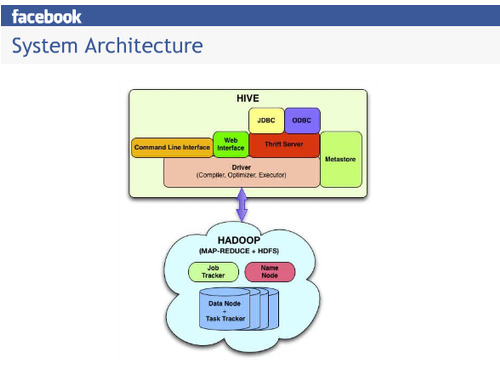
\includegraphics[width=300px,height=200px]{img/hive2.png}
  \caption{Facebook Data Infrastructure\newline
  Fonte: http://nosql.mypopescu.com/post/681603154/presentation-hive-a-petabyte-scale-data-warehouse}
  \label{hive}
\end{figure}
 
Atualmente, existem três formatos de arquivos suportados no Hive, que são
textfile, SEQUENCEFILE e RCFILE.


\section{\textbf{Proposta de transformação de Data Warehouse em um modelo 
            de armazenamento chave-valor}}

Uma abordagem possível para nossa solução seria baseada em ATL (model
transformation technology), consiste em realizar transformações usando modelos,
essa abordagem facilita na automatização do processo de transformação, além de
ter suporte de ferramentas e APIs.

Para realizar transformações entre modelos é necessário criar correspondência
entre elementos de um modelo com elementos do outro modelo, segundo \cite{Didonet}.
Essa correspondência é realizada através de regras de associação. Em nosso
ambiente é necessário associar as tabelas, atributos, associações, funções de
carregamento e demais componentes da arquitetura do BD do ProInfoData, a
elementos correspondentes no modelo do Hadoop, Hive e MapReduce.

No BD do ProInfoData existem tabelas de dimensão e tabelas fatos, inicialmente
temos que criar regras de transformação para associar as tabelas essências do
DW ao modelo de armazenamento do hadoop.

Um dos formatos que o hadoop suporta é o arquivo de texto, transformaremos as
tabelas fatos e tabelas de dimensão em um arquivo, onde um tupla corresponde a
uma linha e cada atributo das tabelas corresponderia a um campo do arquivo. Uma
possível dificuldade seria representar as associações entre as tabelas fatos e
as tabelas de dimensão, no DW essa associação ocorre com chaves primárias e
estrangeiras. Para resolver esse problema teremos que inserir no arquivo todos
os atributos das tabelas associadas, esta abordagem pode impactar diretamente no
tamanho do arquivo, mas esse problema não é preocupando, uma vez que o MapReduce
foi projetado para suportar grande volume de dados, na faixa de terabytes e até
pentabytes.

Então uma ou mais tabelas corresponderiam a um arquivo de texto, suas linhas a
concatenação das tuplas associadas às tabelas e os campos do arquivo
corresponderiam a atributos das tabelas.

Um arquivo de armazenamento teria os campos correspondendo as colunas de
algumas tabelas do BD do ProInfoData. Como exemplo o arquivo denominado
"arq-disponibilidade", ele tem os campos: \textbf{Mac-Address} identificador
da máquina, \textbf{INEP} código identificador da escola, \textbf{Nome da Escola},
\textbf{Cidade}, \textbf{Estado}, \textbf{Região} e \textbf{Data de contato} dia em
que a máquina se comunicou, conforme abaixo:

\textbf{MAC-ADDRESS, INEP, NOME-ESCOLA, CIDADE, ESTADO, REGIÃO, DATA-CONTATO}\\

A staging area seria transformada em um arquivo, pois é uma tabela simples de
armazenamento temporário, poderiam ser criadas rotinas de atualização dos
arquivos de armazenamento permanente a partir do arquivo da staging area. Na
verdade teria que ser estudado melhor a própria existência do arquivo de
armazenamento temporário, pois outra solução seria inserir os novos dados vindos
do servidor WebService diretamente nos arquivos de armazenamento, com isso
evitaria a manutenção do arquivo temporário. Essa abordagem tornaria o processo
mais automatizado, pois se houvesse algum incremento ou alteração na
estrutura do arquivo temporário, essa modificação impactaria nas rotinas de
atualização que precisariam ser adaptadas.
 
Essa última abordagem sem o armazenamento temporário eliminaria a etapa de
carregamento dos dados, contudo teria que ser avaliado o desempenho de inserções
nos arquivos de armazenamento, mesmo se existir o arquivo temporário também será
necessário testar o desempenho de inserções nele.

O carregamento do DW tem como tarefa principalmente a classificação dos dados,
ele realiza o catálogo de hardware, associa as máquinas as sua escola
correspondente e também associa a disponibilidade com a data de contato, além de
detectar alteração de hardware. Essa etapa corresponde às funções de Map, ou
seja, o mapeamento dos dados é responsável por essas classificações, já que o
objetivo inerente do mapeamento é descrever o modelo dos dados, consequentemente
essa tarefa será de responsabilidade do programador quando escrever as funções
de Map.

Outra etapa importante é a agregação e sumarização dos dados no conjunto de DM,
essa etapa é uma das mais cruciais, pois impacta diretamente no desempenho do
DW, ela corresponde as funções de Reduce, pois no Reduce podemos
agregar vários Maps, ou seja, as entradas dos arquivos de armazenamento são
mapeadas e repassadas ao Reduce para manipular os resultados. Desta forma os DM
não existiriam mais, o programador assume toda responsabilidade ao escrever as
funções de Reduce conforme a necessidade das consultas.

As consultas são de responsabilidade do Hive que oferece uma interface para
recuperação dos dados, esse é um ponto de extrema importância, pois o Hive não
implementa todas as funções SQL, dependendo da consulta o programador terá que
escrevê-la manualmente.

Um código protótipo de uma função MapReduce usando o arquivo
“arq-disponibilidade” seria:

\lstinputlisting[language=java, label=teste, caption={Disponibilidade por região}]{Availability.java}

Este código implementa uma função Map e uma função Reduce. O Map recebe como entrada
o arq-disponibilidade, onde a linha é chave e seu conteúdo o valor, gera uma saída
intermediária para o Reduce com os campo data(chave) e região(valor). O Reduce,
por sua vez, agrega a disponibilidade por regiões do Brasil, e gera como saída
o par data(chave) e região seguida pelo quantidade de máquinas(valor).

Nota-se na linha 138 foi definida esplicitamente a quantidade de Reduce, nesse caso
somente uma máquina realizará todo o processo, pois foi implementado para um ambiente
de teste inicial.

\section{\textbf{Discussão}}
Pode-se notar que a implementação das funções Map e Reduce é bastante simples,
permitindo que o programador se atenha apenas a geração dos dados, sem preocupar-se
com a comunicação entre nós.

A simplicidade na codificação MapReduce e no armazenamento do Hadoop torna a
transformação mais fácil, pois é necessário apenas associar elementos
dos dois modelos, no nosso caso ocorrerão as seguintes transformações: tabelas serão
mapeadas em arquivos, tuplas corresponderão a linha dos arquivos, os atributos a 
campos dos arquivos, as funções de carregamento corresponderão as funções Map, as 
funções de agregação (carregamento dos DMs) funções Reduce e as consultas serão
realizadas pelo Hive.

Pontos importantes ainda a sererem estudados, são as consultas feitas pelo Hive
e a migração dos dados da base do ProInfoData, mas essa parte focaremos na
continuação desse trabalho. 

\bibliographystyle{plain}
\bibliography{tg}
\end{document}
